\chapter{Fundamentos Teóricos da Qualidade Baseada em Tarefa}
\label{chap:fundamentacao}

\section{Teoria de Detecção de Sinais e Tomada de Decisão Estatística}
\label{sec:sdt}

A Teoria de Detecção de Sinais (SDT), originada na engenharia de telecomunicações e adaptada para a física médica, fornece a estrutura matemática para modelar o processo de diagnóstico médico sob condições de incerteza estocástica \cite{peterson1954, lusted1968, metz1986, barrett_myers_2004}.

Em termos clínicos, quando um radiologista avalia uma região anatômica em um exame de tomografia, ele se depara com duas situações mutuamente exclusivas: ou o paciente não apresenta lesão naquele ponto (hipótese nula, $H_0$), ou existe uma lesão de contraste e morfologia definidos sobreposta às estruturas normais (hipótese alternativa, $H_1$).

Matematicamente, representamos a imagem digital através de um vetor de dados $\mathbf{g} \in \mathbb{R}^N$, formado por $N = N_x \times N_y$ pixels ordenados sequencialmente. O teste de hipóteses binário é formalizado por:
\begin{equation}
  \begin{cases}
    H_0 : \mathbf{g} = \mathbf{b} & \text{(Sinal Ausente: Apenas Ruído e Fundo Anatômico)} \\
    H_1 : \mathbf{g} = \mathbf{b} + \mathbf{s} & \text{(Sinal Presente: Lesão } \mathbf{s} \text{ Sobreposta ao Fundo } \mathbf{b}\text{)}
  \end{cases}
  \label{eq:hipoteses_sdt}
\end{equation}

Um observador (seja um especialista humano ou um modelo computacional) avalia a imagem aplicando um operador matemático $t(\mathbf{g}): \mathbb{R}^N \to \mathbb{R}$, que condensa todas as informações visuais em um único valor numérico escalar $t$, denominado estatística de teste.

A decisão diagnóstica é tomada comparando $t$ com um valor limiar de corte $t_c$:
\begin{itemize}
  \item Se $t \ge t_c$, o observador conclui que a lesão está presente ($H_1$);
  \item Se $t < t_c$, o observador declara que a imagem é normal ($H_0$).
\end{itemize}

Como a imagem contém ruído estocástico, a estatística $t$ comporta-se como uma variável aleatória, gerando duas curvas de densidade de probabilidade: $p(t|H_0)$ e $p(t|H_1)$, conforme ilustrado no Painel A da \cref{fig:sdt_roc_2afc}.

\begin{figure}[htbp]
  \centering
  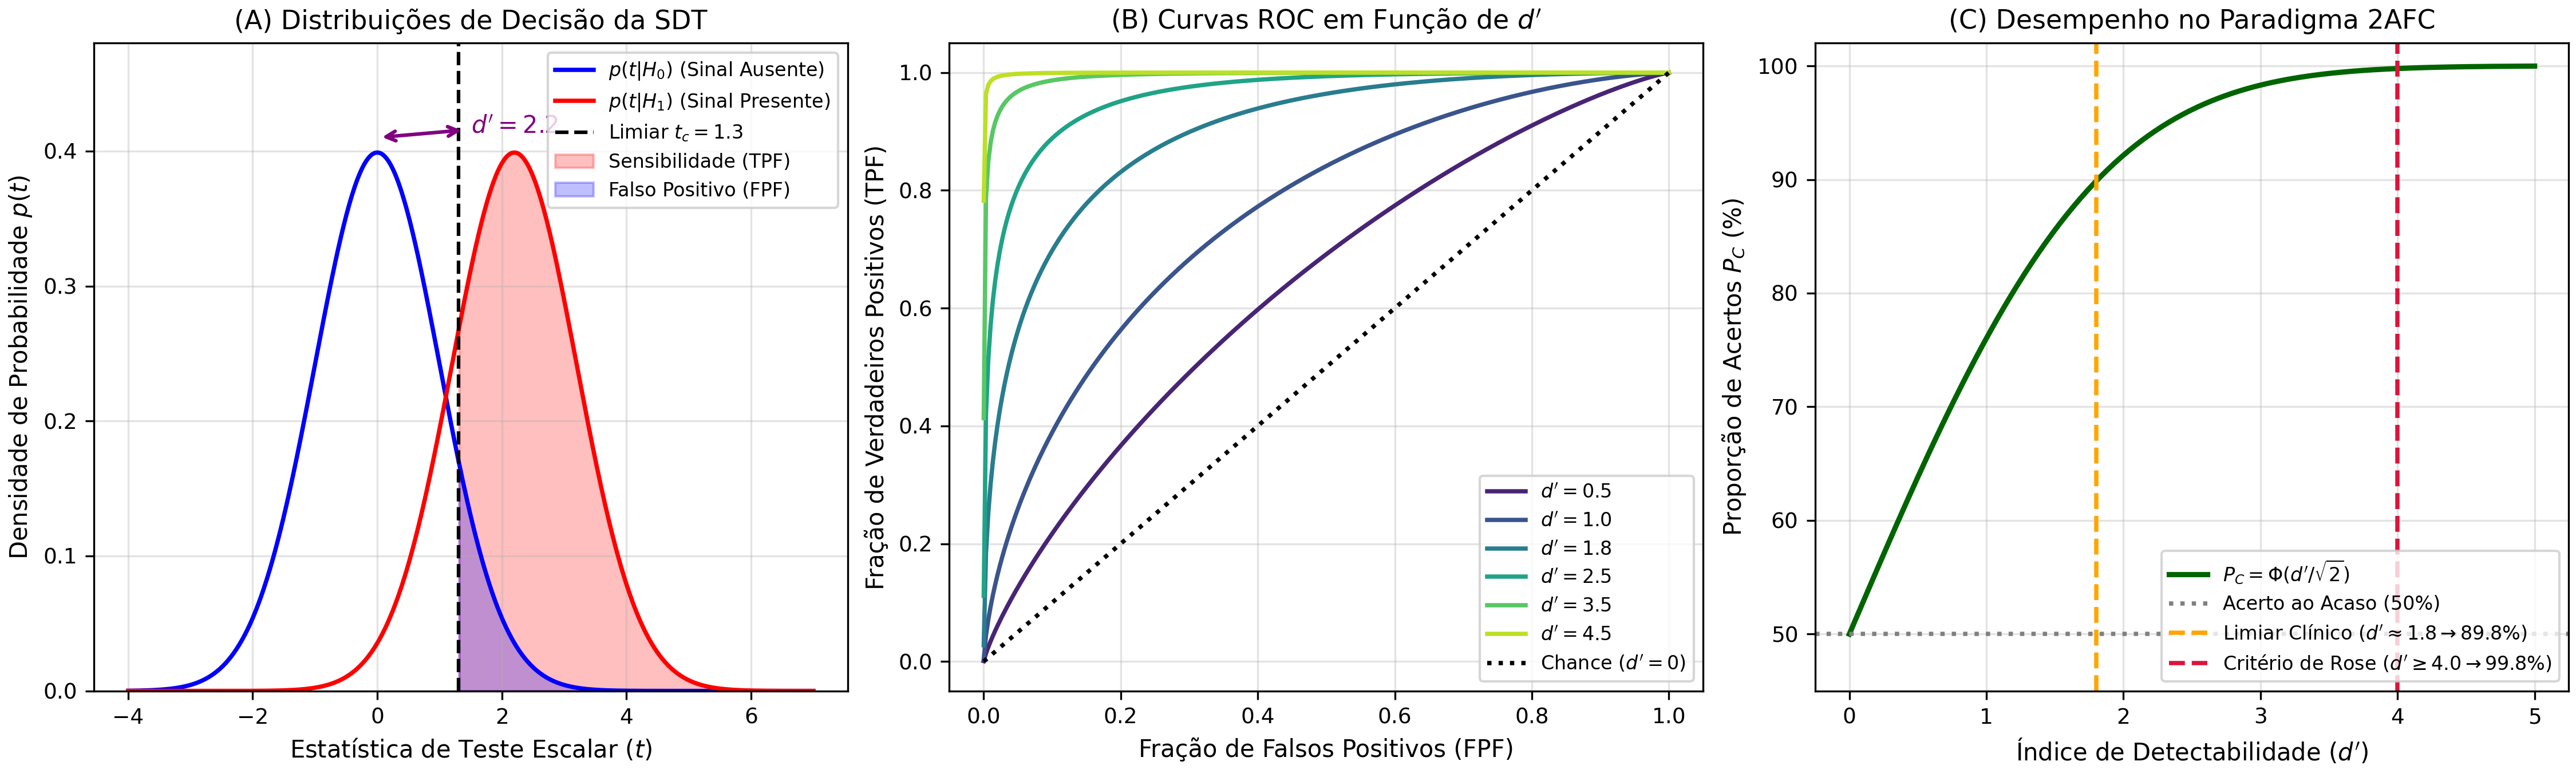
\includegraphics[width=0.98\textwidth]{figuras/fig1_sdt_roc_2afc.png}
  \caption{Fundamentos da Teoria de Detecção de Sinais (SDT), Curvas ROC e Psicofísica 2AFC. (A) Distribuições condicionais de probabilidade $p(t|H_0)$ e $p(t|H_1)$, ilustrando o limiar de decisão $t_c$, a taxa de verdadeiros positivos (TPF) e falsos positivos (FPF), e a separação $d'$. (B) Família de curvas ROC para diferentes índices de detectabilidade ($d' = 0{,}5$ a $4{,}5$). (C) Relação psicofísica formal $P_C = \Phi(d'/\sqrt{2})$ no paradigma 2AFC, destacando o limiar clínico e o critério de Rose.}
  \label{fig:sdt_roc_2afc}
\end{figure}

A variação do limiar $t_c$ permite construir a curva Característica de Operação do Receptor (curva ROC), cujas ordenadas representam a Fração de Verdadeiros Positivos (TPF ou Sensibilidade) e as abscissas indicam a Fração de Falsos Positivos (FPF ou $1 - \text{Especificidade}$) \cite{metz1986}:
\begin{equation}
  \text{TPF}(t_c) = \int_{t_c}^{\infty} p(t|H_1) \, dt, \qquad \text{FPF}(t_c) = \int_{t_c}^{\infty} p(t|H_0) \, dt
  \label{eq:tpf_fpf}
\end{equation}

A integral sob a curva ROC define a métrica global de acurácia, denominada Área sob a Curva ROC (AUC), que varia de $0{,}5$ (desempenho equivalente ao acaso puro) até $1{,}0$ (discriminação perfeita sem erros).

\section{O Índice de Detectabilidade no Domínio Espacial}
\label{sec:dprime_espacial}

Quando as distribuições condicionais $p(t|H_0)$ e $p(t|H_1)$ são gaussianas com variâncias semelhantes, a separação estatística entre elas é sintetizada pelo Índice de Detectabilidade ($d'$):
\begin{equation}
  d' = \frac{\langle t | H_1 \rangle - \langle t | H_0 \rangle}{\sqrt{\frac{1}{2}\sigma^2(t|H_1) + \frac{1}{2}\sigma^2(t|H_0)}}
  \label{eq:dprime_definicao}
\end{equation}

Para a classe dos observadores lineares, a estatística $t$ é obtida pelo produto interno entre a imagem $\mathbf{g}$ e um vetor de template (filtro linear) $\mathbf{w} \in \mathbb{R}^N$:
\begin{equation}
  t = \mathbf{w}^T \mathbf{g} = \sum_{i=1}^N w_i g_i
  \label{eq:template_linear}
\end{equation}

Substituindo essa relação linear na definição de $d'$:
\begin{itemize}
  \item O valor esperado sob $H_0$ é $\langle t | H_0 \rangle = \mathbf{w}^T \langle \mathbf{b} \rangle$;
  \item O valor esperado sob $H_1$ é $\langle t | H_1 \rangle = \mathbf{w}^T \langle \mathbf{b} \rangle + \mathbf{w}^T \mathbf{s}$;
  \item A diferença entre as médias das hipóteses é dada por $\Delta \langle t \rangle = \mathbf{w}^T \mathbf{s}$;
  \item A variância do teste para ruído de matriz de covariância $\mathbf{K} = \langle (\mathbf{b} - \langle \mathbf{b} \rangle)(\mathbf{b} - \langle \mathbf{b} \rangle)^T \rangle$ é $\sigma^2(t) = \mathbf{w}^T \mathbf{K} \mathbf{w}$.
\end{itemize}

Assim, obtém-se a formulação geral do índice de detectabilidade linear no domínio espacial:
\begin{equation}
  d' = \frac{\mathbf{w}^T \mathbf{s}}{\sqrt{\mathbf{w}^T \mathbf{K} \mathbf{w}}}
  \label{eq:dprime_linear_espacial}
\end{equation}

Em termos intuitivos, o numerador ($\mathbf{w}^T \mathbf{s}$) quantifica quanta energia útil do sinal o filtro $\mathbf{w}$ consegue capturar, enquanto o denominador ($\sqrt{\mathbf{w}^T \mathbf{K} \mathbf{w}}$) mede a quantidade de ruído indesejado que atravessa esse mesmo filtro. O valor de $d'$ representa, portanto, a relação sinal-ruído efetiva do observador na tarefa.

\section{Transição para o Domínio das Frequências via Teorema de Wiener-Khinchin}
\label{sec:wiener_khinchin}

A manipulação da matriz de covariância $\mathbf{K}$ no domínio espacial torna-se computacionalmente inviável para imagens de alta resolução (onde $N \approx 262.144$ pixels).

Entretanto, se o ruído de fundo for estacionário no sentido amplo (WSS), a autocorrelação entre dois pontos espaciais depende exclusivamente da distância relativa entre eles. Matematicamente, isso transforma a matriz de covariância em uma matriz circulante.

Pelo Teorema de Wiener-Khinchin, a Transformada de Fourier bidimensional da função de autocorrelação espacial é exatamente igual à densidade espectral de potência do ruído, denominada Espectro de Potência do Ruído ($NPS(u, v)$) \cite{barrett_myers_2004, wagner1979}. Essa propriedade permite transpor o cálculo de $d'$ para integrais contínuas no domínio das frequências espaciais.

A \cref{fig:spectral_metrics} ilustra as quatro grandezas espectrais que compõem o cálculo da detectabilidade.

\begin{figure}[htbp]
  \centering
  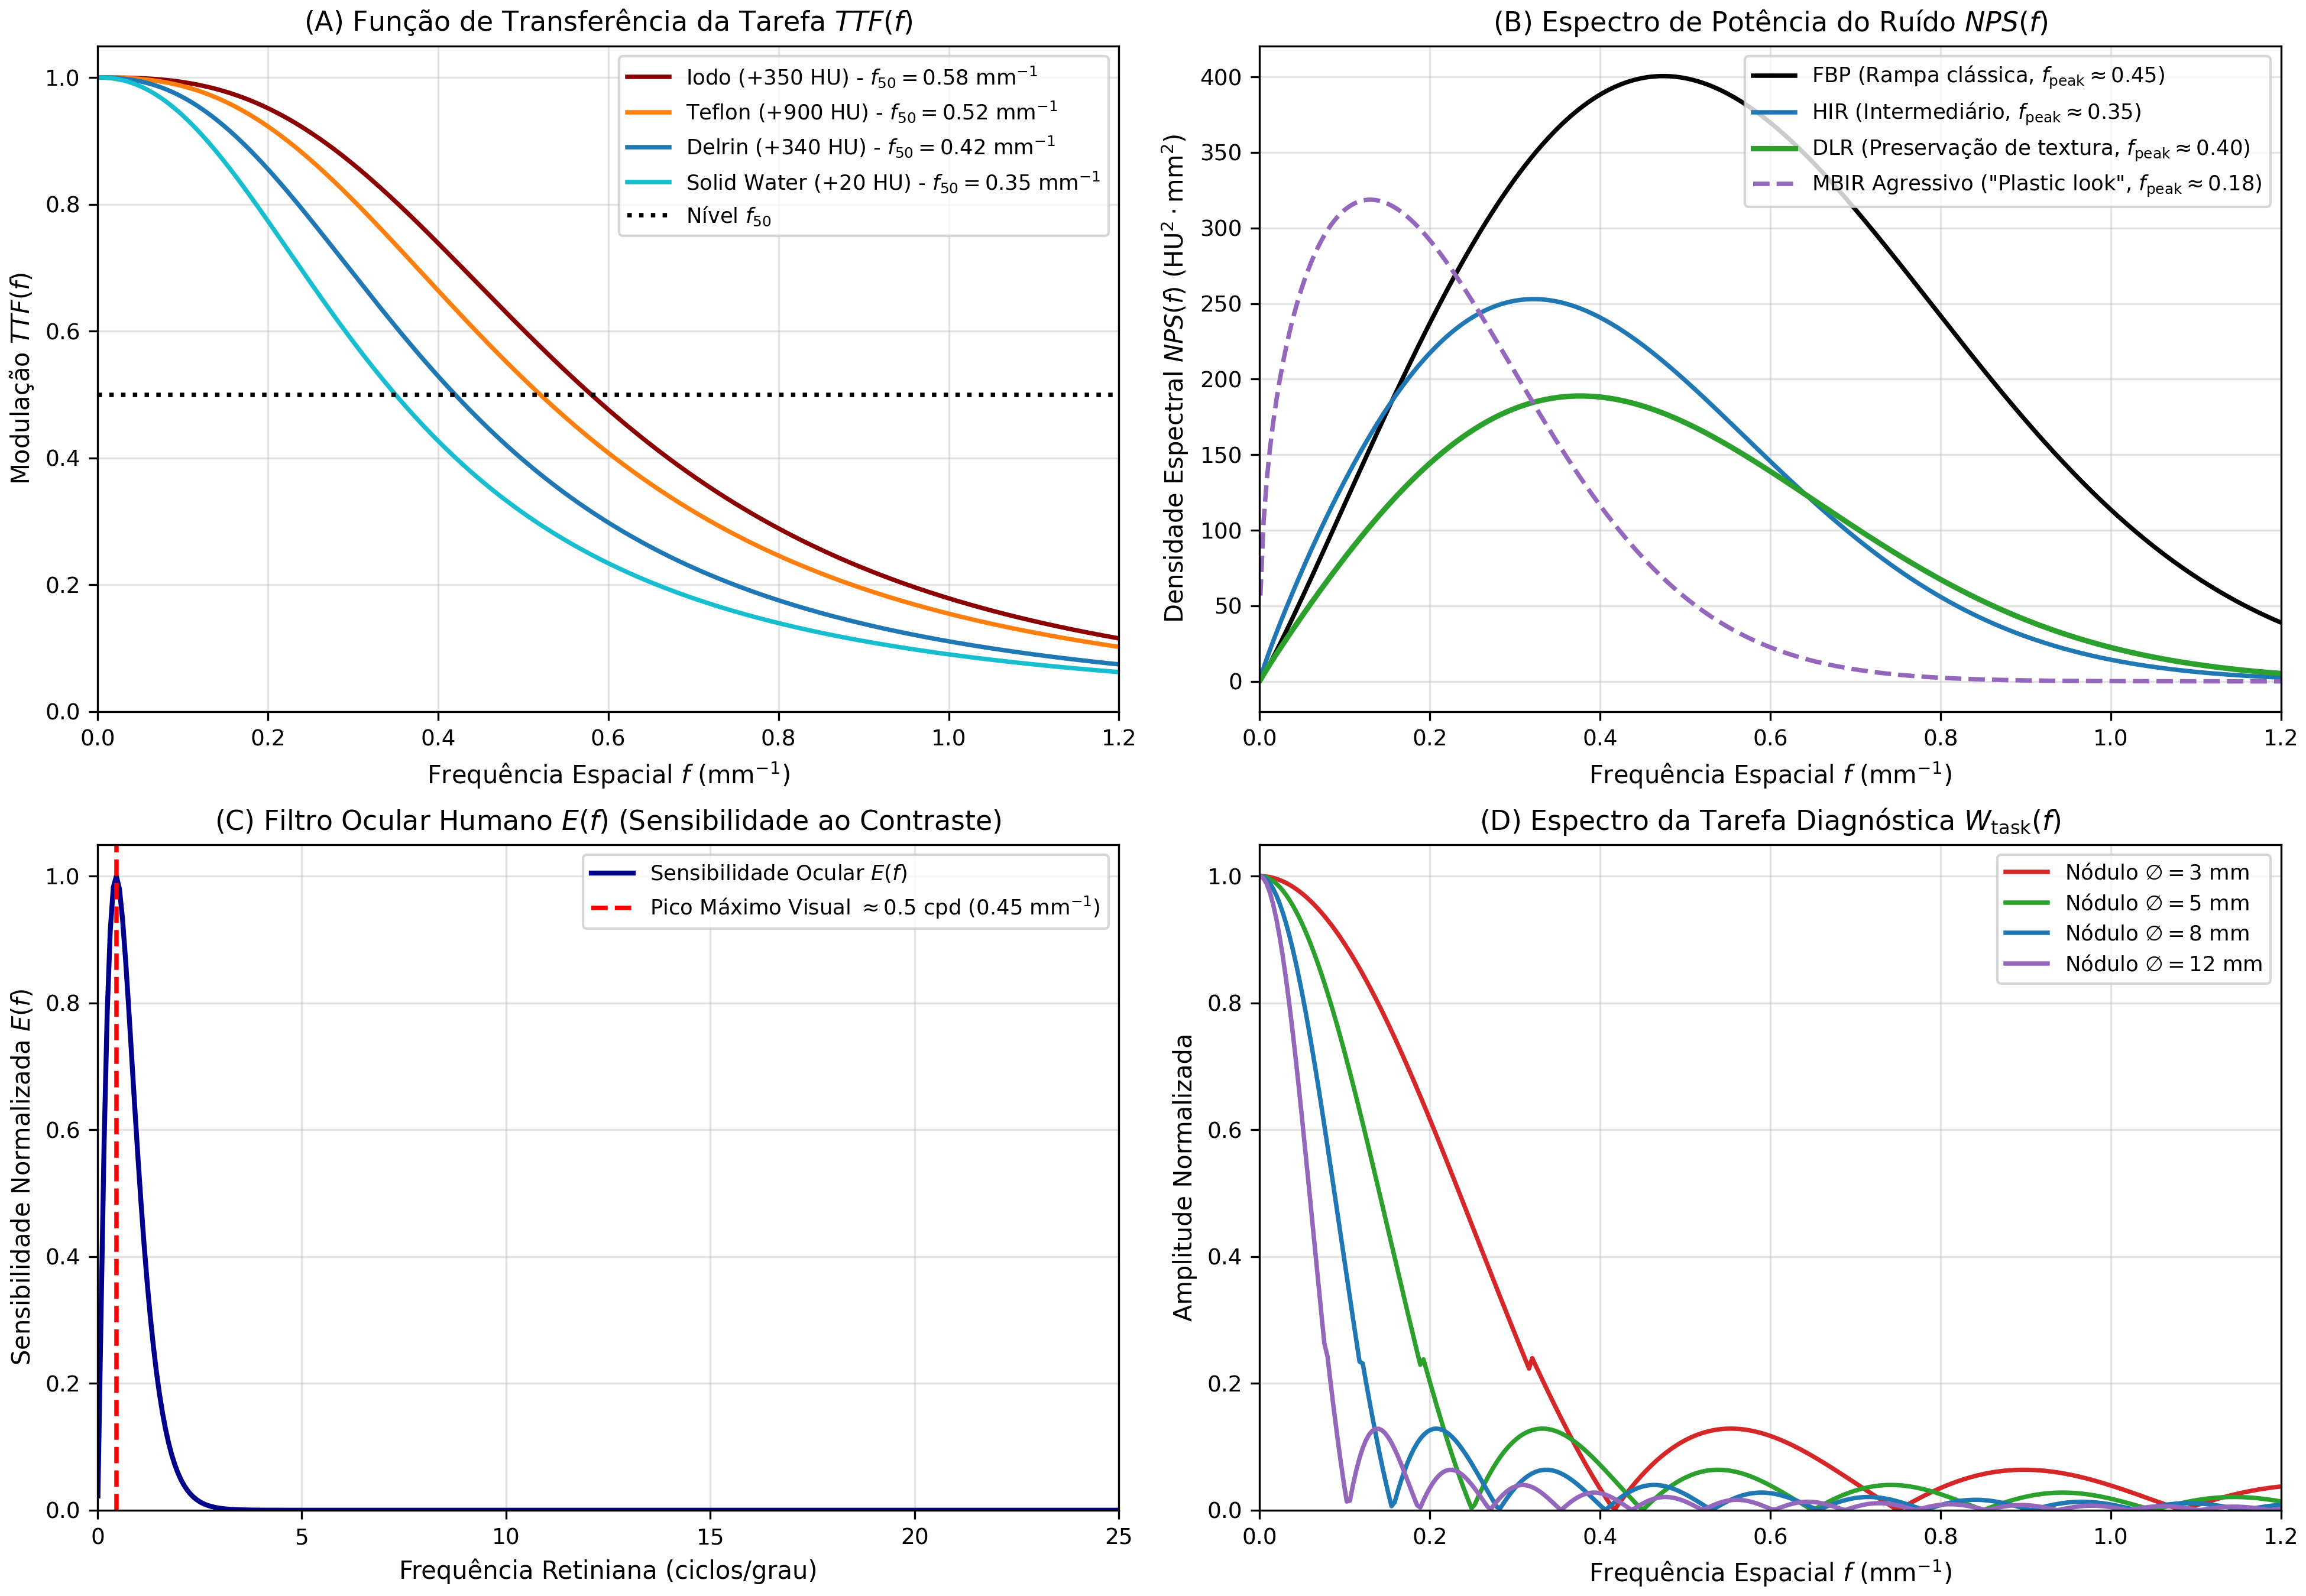
\includegraphics[width=0.98\textwidth]{figuras/fig2_spectral_metrics.png}
  \caption{Métricas Espectrais de Qualidade de Imagem Baseada em Tarefas. (A) Função de Transferência da Tarefa $TTF(f)$ para insertos de diferentes contrastes e materiais, evidenciando a dependência não linear e o ponto de modulação de 50\% ($f_{50}$). (B) Espectro de Potência do Ruído $NPS(f)$ comparando FBP (rampa de alta frequência), HIR, DLR e MBIR com deslocamento de $f_{\text{peak}}$ (``plastic look''). (C) Filtro Ocular Humano $E(f)$ (Função de Sensibilidade ao Contraste). (D) Espectro de Potência da Tarefa Diagnóstica $W_{\text{task}}(f)$ para lesões nodulares esféricas de diferentes diâmetros ($\varnothing = 3, 5, 8, 12\text{ mm}$).}
  \label{fig:spectral_metrics}
\end{figure}

\subsection{Função de Transferência da Tarefa e Resolução Dependente de Contraste}
A Função de Transferência da Tarefa ($TTF(f)$) quantifica a resolução espacial do tomógrafo para um contraste radiológico e nível de dose específicos \cite{aapm_tg233_2019}. Ela é obtida experimentalmente através da técnica da borda circular em insertos cilíndricos de calibração (Painel A da \cref{fig:spectral_metrics}).

O cálculo segue três etapas analíticas:
\begin{enumerate}
  \item Obtenção do perfil radial de atenuação em torno do centro geométrico do inserto, gerando a Função de Resposta ao Degrau Radial ($\text{ESF}(r)$);
  \item Diferenciação numérica radial para obter a Função de Espalhamento de Linha:
  \begin{equation}
    \text{LSF}(r) = \frac{d}{dr}\text{ESF}(r)
    \label{eq:lsf}
  \end{equation}
  \item Cálculo da Transformada de Fourier 1D normalizada na frequência zero:
  \begin{equation}
    TTF(f) = \frac{\left| \int_{-\infty}^{\infty} \text{LSF}(r) e^{-i 2\pi f r} \, dr \right|}{\left| \int_{-\infty}^{\infty} \text{LSF}(r) \, dr \right|}
    \label{eq:ttf_formula}
  \end{equation}
\end{enumerate}

A frequência $f_{50}$ representa o ponto no qual a transferência de contraste decai para 50\% do valor máximo, servindo como índice de nitidez do protocolo.

\subsection{Espectro de Potência do Ruído e Textura Espacial}
O Espectro de Potência do Ruído 2D ($NPS(u, v)$) quantifica como a energia do ruído estocástico se distribui pelas frequências espaciais da imagem:
\begin{equation}
  NPS(u, v) = \frac{\Delta x \Delta y}{N_x N_y} \left\langle \left| \mathcal{F}_{2D} \left\{ I(x, y) - \overline{I}(x, y) \right\} \right|^2 \right\rangle
  \label{eq:nps_formula}
\end{equation}
onde $\overline{I}(x, y)$ é a superfície de fundo removida por \emph{detrending}.

Para caracterizar a textura visual do ruído, calcula-se a frequência de pico ($f_{\text{peak}}$) e a frequência média ponderada ($f_{\text{av}}$):
\begin{equation}
  f_{\text{av}} = \frac{\int_{0}^{\infty} f \cdot NPS(f) \, df}{\int_{0}^{\infty} NPS(f) \, df}
  \label{eq:fav}
\end{equation}

Conforme demonstrado no Painel B da \cref{fig:spectral_metrics}, algoritmos analíticos (FBP) apresentam picos em frequências mais elevadas (textura granular fina), enquanto métodos iterativos agressivos deslocam o pico para frequências baixas, provocando perda de textura estocástica natural (\emph{plastic look}).

\subsection{Filtro Ocular e Modelagem Biofísica da Visão Humana}
O olho humano não responde de forma uniforme a todas as frequências espaciais. A Função de Sensibilidade ao Contraste do sistema visual atua como um filtro passa-faixa, modelado matematicamente pelo Filtro Ocular $E(f)$ \cite{burgess1994, aapm_tg233_2019}:
\begin{equation}
  E(f) = \left( \frac{f}{f_0} \right)^n \exp\left[ -c \left( \frac{f}{f_0} \right)^m \right]
  \label{eq:eye_filter}
\end{equation}
com parâmetros $f_0 = 0{,}8 \text{ cpd}$, $n = 1{,}3$, $m = 1{,}1$ e $c = 2{,}2$.

A frequência angular na retina ($f_{\text{retina}}$, em ciclos por grau) relaciona-se com a frequência espacial física na imagem ($f_{\text{imagem}}$, em $\text{mm}^{-1}$) para uma distância de visualização de $500 \text{ mm}$ através da expressão:
\begin{equation}
  f_{\text{retina}} (\text{ciclos/grau}) \approx 8{,}727 \cdot f_{\text{imagem}} (\text{mm}^{-1})
  \label{eq:fretina}
\end{equation}

O Painel C da \cref{fig:spectral_metrics} evidencia que o olho humano possui máxima sensibilidade a variações de contraste na faixa de 3 a 5 ciclos/grau ($\approx 0{,}45 \text{ mm}^{-1}$ no plano do monitor diagnóstico), atenuando tanto variações muito suaves quanto detalhes ultrafinos.

Adicionalmente, a fisiologia da visão introduz um ruído interno neural ($\sigma_{\text{int}}^2$), de modo que a detectabilidade humana real relaciona-se com o modelo computacional por:
\begin{equation}
  d'_{\text{humano}} = \frac{d'_{\text{NPWE}}}{\sqrt{1 + \left(\frac{\sigma_{\text{int}}}{\sigma_{\text{ext}}}\right)^2}}
  \label{eq:dprime_humano_int}
\end{equation}

\subsection{Espectro da Tarefa Diagnóstica e o Critério de Rose}
Para uma lesão circular homogênea de raio $R$ e contraste central $\Delta C$, o espectro da tarefa diagnóstica no domínio de Fourier é descrito por uma função de Bessel ordinária de primeira espécie $J_1$:
\begin{equation}
  W_{\text{task}}(f) = \Delta C \cdot 2\pi R^2 \left| \frac{J_1(2\pi R f)}{2\pi R f} \right|
  \label{eq:wtask}
\end{equation}

O Painel D da \cref{fig:spectral_metrics} mostra que lesões maiores concentram sua energia em frequências espaciais baixas, enquanto lesões puntiformes dispersam sua informação em frequências médias e altas.

O Critério clássico de Rose \cite{rose1948} postulava que um sinal só é detectado pelo ser humano se a relação de contraste-ruído ponderada pela área for superior a 5 ($k \ge 5$). Na formulação contemporânea da TBIQ, esse limiar corresponde a $d' \ge 4{,}0 \text{ a } 5{,}0$ para detecção quase certa ($P_C \ge 99\%$), enquanto $d' \approx 1{,}5 \text{ a } 2{,}0$ estabelece o limite de visibilidade clínica aceitável.

\section{Paradigmas de Detecção e a Dedução Matemática do Experimento 2AFC}
\label{sec:2afc_deducao}

O padrão-ouro experimental para medir a percepção humana em física médica é o experimento de Escolha Forçada entre Duas Alternativas (2AFC) \cite{burgess2011, eckstein2000}.

No teste 2AFC, apresentam-se ao leitor dois campos de imagem idênticos: um contendo apenas ruído ($H_0$) e outro contendo a lesão inserida sobre o ruído ($H_1$). O observador avalia as duas imagens e calcula suas respectivas variáveis de decisão: $t_0 = t(\mathbf{g}|H_0)$ e $t_1 = t(\mathbf{g}|H_1)$. O observador acerta a escolha se $t_1 > t_0$.

Considerando que $t_0 \sim \mathcal{N}(\mu_0, \sigma^2)$ e $t_1 \sim \mathcal{N}(\mu_1, \sigma^2)$ são variáveis normais independentes, definimos a variável de diferença $\Delta t = t_1 - t_0$.

As propriedades estatísticas dessa variável combinada são:
\begin{itemize}
  \item Média da diferença: $\mu_{\Delta t} = \mu_1 - \mu_0$;
  \item Variância da diferença: $\sigma_{\Delta t}^2 = \sigma^2(t_1) + \sigma^2(t_0) = 2\sigma^2$;
  \item Desvio padrão da diferença: $\sigma_{\Delta t} = \sqrt{2}\sigma$.
\end{itemize}

A proporção de acertos esperada ($P_C$) é a probabilidade de que $\Delta t > 0$:
\begin{equation}
  P_C = P(\Delta t > 0) = P\left( \frac{\Delta t - \mu_{\Delta t}}{\sigma_{\Delta t}} > \frac{-(\mu_1 - \mu_0)}{\sqrt{2}\sigma} \right) = \Phi\left( \frac{\mu_1 - \mu_0}{\sqrt{2}\sigma} \right)
  \label{eq:pc_2afc_step}
\end{equation}

Como $d' = \frac{\mu_1 - \mu_0}{\sigma}$, estabelece-se a relação fundamental da psicofísica 2AFC:
\begin{equation}
  P_C = \Phi\left( \frac{d'}{\sqrt{2}} \right)
  \label{eq:pc_dprime_2afc}
\end{equation}

Invertendo a equação através da função cumulativa normal inversa $\Phi^{-1}$:
\begin{equation}
  d'_{\text{humano}} = \sqrt{2} \cdot \Phi^{-1}(P_C)
  \label{eq:dprime_humano_inversa}
\end{equation}

Essa dedução demonstra a origem física do fator $\sqrt{2}$, permitindo converter a porcentagem de acertos de médicos radiologistas em um índice escalar de detectabilidade $d'$ diretamente comparável aos modelos matemáticos.
